% Options for packages loaded elsewhere
\PassOptionsToPackage{unicode}{hyperref}
\PassOptionsToPackage{hyphens}{url}
%
\documentclass[
]{article}
\usepackage{amsmath,amssymb}
\usepackage{lmodern}
\usepackage{iftex}
\ifPDFTeX
  \usepackage[T1]{fontenc}
  \usepackage[utf8]{inputenc}
  \usepackage{textcomp} % provide euro and other symbols
\else % if luatex or xetex
  \usepackage{unicode-math}
  \defaultfontfeatures{Scale=MatchLowercase}
  \defaultfontfeatures[\rmfamily]{Ligatures=TeX,Scale=1}
\fi
% Use upquote if available, for straight quotes in verbatim environments
\IfFileExists{upquote.sty}{\usepackage{upquote}}{}
\IfFileExists{microtype.sty}{% use microtype if available
  \usepackage[]{microtype}
  \UseMicrotypeSet[protrusion]{basicmath} % disable protrusion for tt fonts
}{}
\makeatletter
\@ifundefined{KOMAClassName}{% if non-KOMA class
  \IfFileExists{parskip.sty}{%
    \usepackage{parskip}
  }{% else
    \setlength{\parindent}{0pt}
    \setlength{\parskip}{6pt plus 2pt minus 1pt}}
}{% if KOMA class
  \KOMAoptions{parskip=half}}
\makeatother
\usepackage{xcolor}
\usepackage[margin=1in]{geometry}
\usepackage{color}
\usepackage{fancyvrb}
\newcommand{\VerbBar}{|}
\newcommand{\VERB}{\Verb[commandchars=\\\{\}]}
\DefineVerbatimEnvironment{Highlighting}{Verbatim}{commandchars=\\\{\}}
% Add ',fontsize=\small' for more characters per line
\usepackage{framed}
\definecolor{shadecolor}{RGB}{248,248,248}
\newenvironment{Shaded}{\begin{snugshade}}{\end{snugshade}}
\newcommand{\AlertTok}[1]{\textcolor[rgb]{0.94,0.16,0.16}{#1}}
\newcommand{\AnnotationTok}[1]{\textcolor[rgb]{0.56,0.35,0.01}{\textbf{\textit{#1}}}}
\newcommand{\AttributeTok}[1]{\textcolor[rgb]{0.77,0.63,0.00}{#1}}
\newcommand{\BaseNTok}[1]{\textcolor[rgb]{0.00,0.00,0.81}{#1}}
\newcommand{\BuiltInTok}[1]{#1}
\newcommand{\CharTok}[1]{\textcolor[rgb]{0.31,0.60,0.02}{#1}}
\newcommand{\CommentTok}[1]{\textcolor[rgb]{0.56,0.35,0.01}{\textit{#1}}}
\newcommand{\CommentVarTok}[1]{\textcolor[rgb]{0.56,0.35,0.01}{\textbf{\textit{#1}}}}
\newcommand{\ConstantTok}[1]{\textcolor[rgb]{0.00,0.00,0.00}{#1}}
\newcommand{\ControlFlowTok}[1]{\textcolor[rgb]{0.13,0.29,0.53}{\textbf{#1}}}
\newcommand{\DataTypeTok}[1]{\textcolor[rgb]{0.13,0.29,0.53}{#1}}
\newcommand{\DecValTok}[1]{\textcolor[rgb]{0.00,0.00,0.81}{#1}}
\newcommand{\DocumentationTok}[1]{\textcolor[rgb]{0.56,0.35,0.01}{\textbf{\textit{#1}}}}
\newcommand{\ErrorTok}[1]{\textcolor[rgb]{0.64,0.00,0.00}{\textbf{#1}}}
\newcommand{\ExtensionTok}[1]{#1}
\newcommand{\FloatTok}[1]{\textcolor[rgb]{0.00,0.00,0.81}{#1}}
\newcommand{\FunctionTok}[1]{\textcolor[rgb]{0.00,0.00,0.00}{#1}}
\newcommand{\ImportTok}[1]{#1}
\newcommand{\InformationTok}[1]{\textcolor[rgb]{0.56,0.35,0.01}{\textbf{\textit{#1}}}}
\newcommand{\KeywordTok}[1]{\textcolor[rgb]{0.13,0.29,0.53}{\textbf{#1}}}
\newcommand{\NormalTok}[1]{#1}
\newcommand{\OperatorTok}[1]{\textcolor[rgb]{0.81,0.36,0.00}{\textbf{#1}}}
\newcommand{\OtherTok}[1]{\textcolor[rgb]{0.56,0.35,0.01}{#1}}
\newcommand{\PreprocessorTok}[1]{\textcolor[rgb]{0.56,0.35,0.01}{\textit{#1}}}
\newcommand{\RegionMarkerTok}[1]{#1}
\newcommand{\SpecialCharTok}[1]{\textcolor[rgb]{0.00,0.00,0.00}{#1}}
\newcommand{\SpecialStringTok}[1]{\textcolor[rgb]{0.31,0.60,0.02}{#1}}
\newcommand{\StringTok}[1]{\textcolor[rgb]{0.31,0.60,0.02}{#1}}
\newcommand{\VariableTok}[1]{\textcolor[rgb]{0.00,0.00,0.00}{#1}}
\newcommand{\VerbatimStringTok}[1]{\textcolor[rgb]{0.31,0.60,0.02}{#1}}
\newcommand{\WarningTok}[1]{\textcolor[rgb]{0.56,0.35,0.01}{\textbf{\textit{#1}}}}
\usepackage{graphicx}
\makeatletter
\def\maxwidth{\ifdim\Gin@nat@width>\linewidth\linewidth\else\Gin@nat@width\fi}
\def\maxheight{\ifdim\Gin@nat@height>\textheight\textheight\else\Gin@nat@height\fi}
\makeatother
% Scale images if necessary, so that they will not overflow the page
% margins by default, and it is still possible to overwrite the defaults
% using explicit options in \includegraphics[width, height, ...]{}
\setkeys{Gin}{width=\maxwidth,height=\maxheight,keepaspectratio}
% Set default figure placement to htbp
\makeatletter
\def\fps@figure{htbp}
\makeatother
\setlength{\emergencystretch}{3em} % prevent overfull lines
\providecommand{\tightlist}{%
  \setlength{\itemsep}{0pt}\setlength{\parskip}{0pt}}
\setcounter{secnumdepth}{-\maxdimen} % remove section numbering
\ifLuaTeX
  \usepackage{selnolig}  % disable illegal ligatures
\fi
\IfFileExists{bookmark.sty}{\usepackage{bookmark}}{\usepackage{hyperref}}
\IfFileExists{xurl.sty}{\usepackage{xurl}}{} % add URL line breaks if available
\urlstyle{same} % disable monospaced font for URLs
\hypersetup{
  pdftitle={Determinants Elasticity xgbTree},
  hidelinks,
  pdfcreator={LaTeX via pandoc}}

\title{Determinants Elasticity xgbTree}
\author{}
\date{\vspace{-2.5em}2023-04-10}

\begin{document}
\maketitle

Preliminaries: load required packages and perform merges

\begin{verbatim}
## -- Attaching packages --------------------------------------- tidyverse 1.3.2 --
## v ggplot2 3.3.6     v purrr   0.3.4
## v tibble  3.1.7     v dplyr   1.0.9
## v tidyr   1.2.0     v stringr 1.4.0
## v readr   2.1.2     v forcats 0.5.1
## -- Conflicts ------------------------------------------ tidyverse_conflicts() --
## x dplyr::filter() masks stats::filter()
## x dplyr::lag()    masks stats::lag()
## Loading required package: Hmisc
## 
## Loading required package: lattice
## 
## Loading required package: survival
## 
## Loading required package: Formula
## 
## 
## Attaching package: 'Hmisc'
## 
## 
## The following objects are masked from 'package:dplyr':
## 
##     src, summarize
## 
## 
## The following objects are masked from 'package:base':
## 
##     format.pval, units
## 
## 
## 
## Attaching package: 'caret'
## 
## 
## The following object is masked from 'package:survival':
## 
##     cluster
## 
## 
## The following object is masked from 'package:purrr':
## 
##     lift
## 
## 
## 
## Attaching package: 'xgboost'
## 
## 
## The following object is masked from 'package:dplyr':
## 
##     slice
## 
## 
## Loading required package: foreach
## 
## 
## Attaching package: 'foreach'
## 
## 
## The following objects are masked from 'package:purrr':
## 
##     accumulate, when
## 
## 
## Loading required package: iterators
## 
## Loading required package: parallel
## 
## 
## Attaching package: 'pdp'
## 
## 
## The following object is masked from 'package:purrr':
## 
##     partial
\end{verbatim}

\hypertarget{create-weight-manually}{%
\section{create weight manually}\label{create-weight-manually}}

\begin{Shaded}
\begin{Highlighting}[]
\FunctionTok{rm}\NormalTok{(}\AttributeTok{list =} \FunctionTok{ls}\NormalTok{())}
\FunctionTok{library}\NormalTok{(tidyverse)}
\FunctionTok{library}\NormalTok{(readxl)}
\NormalTok{filenames }\OtherTok{\textless{}{-}} \FunctionTok{list.files}\NormalTok{(}\StringTok{"./Ranked Measure Data2"}\NormalTok{)}
\NormalTok{filenames}
\end{Highlighting}
\end{Shaded}

\begin{verbatim}
## [1] "2015.xls" "2016.xls" "2017.xls" "2018.xls" "2019.xls"
\end{verbatim}

\begin{Shaded}
\begin{Highlighting}[]
\NormalTok{RMD }\OtherTok{\textless{}{-}} \FunctionTok{data.frame}\NormalTok{(}\FunctionTok{matrix}\NormalTok{(}\AttributeTok{ncol =} \DecValTok{0}\NormalTok{, }\AttributeTok{nrow =} \DecValTok{0}\NormalTok{))}
\ControlFlowTok{for}\NormalTok{ (filename }\ControlFlowTok{in}\NormalTok{ filenames)\{  }
\NormalTok{   yearnum }\OtherTok{\textless{}{-}} \FunctionTok{gsub}\NormalTok{(}\StringTok{".xls"}\NormalTok{, }\StringTok{""}\NormalTok{, filename)  }
\NormalTok{   RMD }\OtherTok{=}\NormalTok{ RMD }\SpecialCharTok{\%\textgreater{}\%} \FunctionTok{bind\_rows}\NormalTok{(}\FunctionTok{assign}\NormalTok{(}\FunctionTok{paste0}\NormalTok{(}\StringTok{"RMD"}\NormalTok{,yearnum), }\FunctionTok{read\_excel}\NormalTok{(}\FunctionTok{paste0}\NormalTok{(}\StringTok{"./Ranked Measure Data2/"}\NormalTok{, filename), }\AttributeTok{sheet=}\StringTok{"Ranked Measure Data"}\NormalTok{, }\AttributeTok{skip =} \DecValTok{1}\NormalTok{) }\SpecialCharTok{\%\textgreater{}\%}
            \FunctionTok{mutate}\NormalTok{(}\AttributeTok{year=}\NormalTok{yearnum) }\SpecialCharTok{\%\textgreater{}\%} 
            \FunctionTok{select}\NormalTok{(FIPS, year, YPLLRateLow, YPLLRateHigh)))}
\NormalTok{\}}
\end{Highlighting}
\end{Shaded}

\begin{verbatim}
## Warning: Expecting numeric in CB3145 / R3145C80: got '^This data was updated on March 29, 2017. Please see http://www.countyhealthrankings.org/content/data-changes for more information.'
\end{verbatim}

\begin{verbatim}
## New names:
## * `Quartile` -> `Quartile...8`
## * `Sample Size` -> `Sample Size...9`
## * `95% CI - Low` -> `95% CI - Low...11`
## * `95% CI - High` -> `95% CI - High...12`
## * `Quartile` -> `Quartile...13`
## * `Sample Size` -> `Sample Size...14`
## * `95% CI - Low` -> `95% CI - Low...16`
## * `95% CI - High` -> `95% CI - High...17`
## * `Quartile` -> `Quartile...18`
## * `Sample Size` -> `Sample Size...19`
## * `95% CI - Low` -> `95% CI - Low...21`
## * `95% CI - High` -> `95% CI - High...22`
## * `Quartile` -> `Quartile...23`
## * `95% CI - Low` -> `95% CI - Low...28`
## * `95% CI - High` -> `95% CI - High...29`
## * `Quartile` -> `Quartile...30`
## * `Sample Size` -> `Sample Size...31`
## * `95% CI - Low` -> `95% CI - Low...33`
## * `95% CI - High` -> `95% CI - High...34`
## * `Quartile` -> `Quartile...35`
## * `95% CI - Low` -> `95% CI - Low...37`
## * `95% CI - High` -> `95% CI - High...38`
## * `Quartile` -> `Quartile...39`
## * `Quartile` -> `Quartile...41`
## * `95% CI - Low` -> `95% CI - Low...43`
## * `95% CI - High` -> `95% CI - High...44`
## * `Quartile` -> `Quartile...45`
## * `Quartile` -> `Quartile...48`
## * `Sample Size` -> `Sample Size...49`
## * `95% CI - Low` -> `95% CI - Low...51`
## * `95% CI - High` -> `95% CI - High...52`
## * `Quartile` -> `Quartile...53`
## * `Quartile` -> `Quartile...57`
## * `Quartile` -> `Quartile...60`
## * `95% CI - Low` -> `95% CI - Low...64`
## * `95% CI - High` -> `95% CI - High...65`
## * `Quartile` -> `Quartile...66`
## * `95% CI - Low` -> `95% CI - Low...69`
## * `95% CI - High` -> `95% CI - High...70`
## * `Quartile` -> `Quartile...71`
## * `Quartile` -> `Quartile...75`
## * `Quartile` -> `Quartile...79`
## * `# Mental Health Providers` -> `# Mental Health Providers...80`
## * `MHP Rate` -> `MHP Rate...81`
## * `MHP Ratio` -> `MHP Ratio...82`
## * `# Mental Health Providers` -> `# Mental Health Providers...83`
## * `MHP Rate` -> `MHP Rate...84`
## * `MHP Ratio` -> `MHP Ratio...85`
## * `Quartile` -> `Quartile...86`
## * `# Medicare Enrollees` -> `# Medicare Enrollees...87`
## * `95% CI - Low` -> `95% CI - Low...89`
## * `95% CI - High` -> `95% CI - High...90`
## * `Quartile` -> `Quartile...91`
## * `95% CI - Low` -> `95% CI - Low...94`
## * `95% CI - High` -> `95% CI - High...95`
## * `Quartile` -> `Quartile...96`
## * `# Medicare Enrollees` -> `# Medicare Enrollees...97`
## * `95% CI - Low` -> `95% CI - Low...99`
## * `95% CI - High` -> `95% CI - High...100`
## * `Quartile` -> `Quartile...101`
## * `Quartile` -> `Quartile...104`
## * `95% CI - Low` -> `95% CI - Low...108`
## * `95% CI - High` -> `95% CI - High...109`
## * `Quartile` -> `Quartile...110`
## * `Quartile` -> `Quartile...114`
## * `95% CI - Low` -> `95% CI - Low...117`
## * `95% CI - High` -> `95% CI - High...118`
## * `Quartile` -> `Quartile...119`
## * `Quartile` -> `Quartile...123`
## * `95% CI - Low` -> `95% CI - Low...127`
## * `95% CI - High` -> `95% CI - High...128`
## * `Quartile` -> `Quartile...129`
## * `Quartile` -> `Quartile...132`
## * `Quartile` -> `Quartile...135`
## * `95% CI - Low` -> `95% CI - Low...138`
## * `95% CI - High` -> `95% CI - High...139`
## * `Quartile` -> `Quartile...140`
## * `Quartile` -> `Quartile...142`
## * `Quartile` -> `Quartile...145`
## * `95% CI - Low` -> `95% CI - Low...148`
## * `95% CI - High` -> `95% CI - High...149`
## * `Quartile` -> `Quartile...150`
## * `95% CI - Low` -> `95% CI - Low...154`
## * `95% CI - High` -> `95% CI - High...155`
## * `Quartile` -> `Quartile...156`
## * `95% CI - Low` -> `95% CI - Low...159`
## * `95% CI - High` -> `95% CI - High...160`
## * `Quartile` -> `Quartile...161`
\end{verbatim}

\begin{verbatim}
## Warning: Expecting numeric in BX3145 / R3145C76: got '^This data was updated on March 29, 2017. Please see http://www.countyhealthrankings.org/content/data-changes for more information.'
\end{verbatim}

\begin{verbatim}
## New names:
## New names:
## * `Quartile` -> `Quartile...8`
## * `95% CI - Low` -> `95% CI - Low...10`
## * `95% CI - High` -> `95% CI - High...11`
## * `Quartile` -> `Quartile...12`
## * `95% CI - Low` -> `95% CI - Low...14`
## * `95% CI - High` -> `95% CI - High...15`
## * `Quartile` -> `Quartile...16`
## * `95% CI - Low` -> `95% CI - Low...18`
## * `95% CI - High` -> `95% CI - High...19`
## * `Quartile` -> `Quartile...20`
## * `95% CI - Low` -> `95% CI - Low...25`
## * `95% CI - High` -> `95% CI - High...26`
## * `Quartile` -> `Quartile...27`
## * `95% CI - Low` -> `95% CI - Low...29`
## * `95% CI - High` -> `95% CI - High...30`
## * `Quartile` -> `Quartile...31`
## * `95% CI - Low` -> `95% CI - Low...33`
## * `95% CI - High` -> `95% CI - High...34`
## * `Quartile` -> `Quartile...35`
## * `Quartile` -> `Quartile...37`
## * `95% CI - Low` -> `95% CI - Low...39`
## * `95% CI - High` -> `95% CI - High...40`
## * `Quartile` -> `Quartile...41`
## * `Quartile` -> `Quartile...43`
## * `95% CI - Low` -> `95% CI - Low...45`
## * `95% CI - High` -> `95% CI - High...46`
## * `Quartile` -> `Quartile...47`
## * `95% CI - Low` -> `95% CI - Low...51`
## * `95% CI - High` -> `95% CI - High...52`
## * `Quartile` -> `Quartile...53`
## * `Quartile` -> `Quartile...56`
## * `95% CI - Low` -> `95% CI - Low...60`
## * `95% CI - High` -> `95% CI - High...61`
## * `Quartile` -> `Quartile...62`
## * `95% CI - Low` -> `95% CI - Low...65`
## * `95% CI - High` -> `95% CI - High...66`
## * `Quartile` -> `Quartile...67`
## * `Quartile` -> `Quartile...71`
## * `Quartile` -> `Quartile...75`
## * `# Mental Health Providers` -> `# Mental Health Providers...76`
## * `MHP Rate` -> `MHP Rate...77`
## * `MHP Ratio` -> `MHP Ratio...78`
## * `# Mental Health Providers` -> `# Mental Health Providers...79`
## * `MHP Rate` -> `MHP Rate...80`
## * `MHP Ratio` -> `MHP Ratio...81`
## * `Quartile` -> `Quartile...82`
## * `# Medicare Enrollees` -> `# Medicare Enrollees...83`
## * `95% CI - Low` -> `95% CI - Low...85`
## * `95% CI - High` -> `95% CI - High...86`
## * `Quartile` -> `Quartile...87`
## * `95% CI - Low` -> `95% CI - Low...90`
## * `95% CI - High` -> `95% CI - High...91`
## * `Quartile` -> `Quartile...92`
## * `# Medicare Enrollees` -> `# Medicare Enrollees...93`
## * `95% CI - Low` -> `95% CI - Low...95`
## * `95% CI - High` -> `95% CI - High...96`
## * `Quartile` -> `Quartile...97`
## * `Quartile` -> `Quartile...100`
## * `95% CI - Low` -> `95% CI - Low...104`
## * `95% CI - High` -> `95% CI - High...105`
## * `Quartile` -> `Quartile...106`
## * `Quartile` -> `Quartile...110`
## * `95% CI - Low` -> `95% CI - Low...113`
## * `95% CI - High` -> `95% CI - High...114`
## * `Quartile` -> `Quartile...115`
## * `Quartile` -> `Quartile...119`
## * `95% CI - Low` -> `95% CI - Low...123`
## * `95% CI - High` -> `95% CI - High...124`
## * `Quartile` -> `Quartile...125`
## * `Quartile` -> `Quartile...128`
## * `Quartile` -> `Quartile...131`
## * `95% CI - Low` -> `95% CI - Low...134`
## * `95% CI - High` -> `95% CI - High...135`
## * `Quartile` -> `Quartile...136`
## * `Quartile` -> `Quartile...138`
## * `Quartile` -> `Quartile...140`
## * `95% CI - Low` -> `95% CI - Low...143`
## * `95% CI - High` -> `95% CI - High...144`
## * `Quartile` -> `Quartile...145`
## * `95% CI - Low` -> `95% CI - Low...149`
## * `95% CI - High` -> `95% CI - High...150`
## * `Quartile` -> `Quartile...151`
## * `95% CI - Low` -> `95% CI - Low...154`
## * `95% CI - High` -> `95% CI - High...155`
## * `Quartile` -> `Quartile...156`
\end{verbatim}

\begin{verbatim}
## Warning: Expecting logical in CY2096 / R2096C103: got '*'
\end{verbatim}

\begin{verbatim}
## Warning: Expecting logical in CY2125 / R2125C103: got '*'
\end{verbatim}

\begin{verbatim}
## Warning: Expecting logical in CY3145 / R3145C103: got '* An error was found in this data, and corrected data is not currently available.'
\end{verbatim}

\begin{verbatim}
## New names:
## New names:
## * `Quartile` -> `Quartile...7`
## * `95% CI - Low` -> `95% CI - Low...12`
## * `95% CI - High` -> `95% CI - High...13`
## * `Quartile` -> `Quartile...14`
## * `95% CI - Low` -> `95% CI - Low...16`
## * `95% CI - High` -> `95% CI - High...17`
## * `Quartile` -> `Quartile...18`
## * `95% CI - Low` -> `95% CI - Low...20`
## * `95% CI - High` -> `95% CI - High...21`
## * `Quartile` -> `Quartile...22`
## * `95% CI - Low` -> `95% CI - Low...25`
## * `95% CI - High` -> `95% CI - High...26`
## * `Quartile` -> `Quartile...27`
## * `95% CI - Low` -> `95% CI - Low...32`
## * `95% CI - High` -> `95% CI - High...33`
## * `Quartile` -> `Quartile...34`
## * `95% CI - Low` -> `95% CI - Low...36`
## * `95% CI - High` -> `95% CI - High...37`
## * `Quartile` -> `Quartile...38`
## * `Quartile` -> `Quartile...40`
## * `95% CI - Low` -> `95% CI - Low...42`
## * `95% CI - High` -> `95% CI - High...43`
## * `Quartile` -> `Quartile...44`
## * `Quartile` -> `Quartile...46`
## * `95% CI - Low` -> `95% CI - Low...48`
## * `95% CI - High` -> `95% CI - High...49`
## * `Quartile` -> `Quartile...50`
## * `95% CI - Low` -> `95% CI - Low...54`
## * `95% CI - High` -> `95% CI - High...55`
## * `Quartile` -> `Quartile...56`
## * `Quartile` -> `Quartile...59`
## * `95% CI - Low` -> `95% CI - Low...61`
## * `95% CI - High` -> `95% CI - High...62`
## * `Quartile` -> `Quartile...63`
## * `95% CI - Low` -> `95% CI - Low...69`
## * `95% CI - High` -> `95% CI - High...70`
## * `Quartile` -> `Quartile...71`
## * `Quartile` -> `Quartile...75`
## * `Quartile` -> `Quartile...79`
## * `Quartile` -> `Quartile...83`
## * `# Medicare Enrollees` -> `# Medicare Enrollees...84`
## * `95% CI - Low` -> `95% CI - Low...86`
## * `95% CI - High` -> `95% CI - High...87`
## * `Quartile` -> `Quartile...88`
## * `95% CI - Low` -> `95% CI - Low...91`
## * `95% CI - High` -> `95% CI - High...92`
## * `Quartile` -> `Quartile...93`
## * `# Medicare Enrollees` -> `# Medicare Enrollees...96`
## * `95% CI - Low` -> `95% CI - Low...98`
## * `95% CI - High` -> `95% CI - High...99`
## * `Quartile` -> `Quartile...100`
## * `Quartile` -> `Quartile...106`
## * `95% CI - Low` -> `95% CI - Low...110`
## * `95% CI - High` -> `95% CI - High...111`
## * `Quartile` -> `Quartile...112`
## * `Quartile` -> `Quartile...116`
## * `95% CI - Low` -> `95% CI - Low...118`
## * `95% CI - High` -> `95% CI - High...119`
## * `Quartile` -> `Quartile...120`
## * `Quartile` -> `Quartile...127`
## * `95% CI - Low` -> `95% CI - Low...131`
## * `95% CI - High` -> `95% CI - High...132`
## * `Quartile` -> `Quartile...133`
## * `Quartile` -> `Quartile...136`
## * `Quartile` -> `Quartile...139`
## * `95% CI - Low` -> `95% CI - Low...142`
## * `95% CI - High` -> `95% CI - High...143`
## * `Quartile` -> `Quartile...144`
## * `Quartile` -> `Quartile...146`
## * `Quartile` -> `Quartile...148`
## * `95% CI - Low` -> `95% CI - Low...151`
## * `95% CI - High` -> `95% CI - High...152`
## * `Quartile` -> `Quartile...153`
## * `95% CI - Low` -> `95% CI - Low...155`
## * `95% CI - High` -> `95% CI - High...156`
## * `Quartile` -> `Quartile...157`
## * `95% CI - Low` -> `95% CI - Low...163`
## * `95% CI - High` -> `95% CI - High...164`
## * `Quartile` -> `Quartile...165`
\end{verbatim}

\begin{Shaded}
\begin{Highlighting}[]
\NormalTok{RMD}\SpecialCharTok{$}\NormalTok{year}\OtherTok{=}\FunctionTok{as.integer}\NormalTok{(RMD}\SpecialCharTok{$}\NormalTok{year)}
\NormalTok{RMD}\OtherTok{=}\NormalTok{RMD }\SpecialCharTok{\%\textgreater{}\%} \FunctionTok{filter}\NormalTok{(}\FunctionTok{substring}\NormalTok{(FIPS, }\DecValTok{3}\NormalTok{,}\DecValTok{5}\NormalTok{)}\SpecialCharTok{!=}\StringTok{"000"}\NormalTok{)}
\NormalTok{RMD}\OtherTok{=}\NormalTok{RMD }\SpecialCharTok{\%\textgreater{}\%} \FunctionTok{drop\_na}\NormalTok{(FIPS)}
\NormalTok{RMDwide}\OtherTok{=} \FunctionTok{pivot\_wider}\NormalTok{(RMD, }\AttributeTok{id\_cols =}\NormalTok{ FIPS,  }\AttributeTok{names\_from =}\NormalTok{ year, }\AttributeTok{values\_from =} \FunctionTok{c}\NormalTok{(YPLLRateLow, YPLLRateHigh))}

\NormalTok{RMDwide}\SpecialCharTok{$}\NormalTok{range15}\OtherTok{=}\NormalTok{(RMDwide}\SpecialCharTok{$}\NormalTok{YPLLRateHigh\_2015 }\SpecialCharTok{{-}}\NormalTok{ RMDwide}\SpecialCharTok{$}\NormalTok{YPLLRateLow\_2015)}\SpecialCharTok{/}\NormalTok{(}\DecValTok{4}\SpecialCharTok{*}\FloatTok{1.96}\NormalTok{)}
\NormalTok{RMDwide}\SpecialCharTok{$}\NormalTok{irange15}\OtherTok{=}\DecValTok{1}\SpecialCharTok{/}\NormalTok{RMDwide}\SpecialCharTok{$}\NormalTok{range15}
\NormalTok{RMDwide}\SpecialCharTok{$}\NormalTok{weight15}\OtherTok{=}\NormalTok{RMDwide}\SpecialCharTok{$}\NormalTok{irange15 }\SpecialCharTok{/} \FunctionTok{sum}\NormalTok{(RMDwide}\SpecialCharTok{$}\NormalTok{irange15, }\AttributeTok{na.rm =} \ConstantTok{TRUE}\NormalTok{)}
\FunctionTok{sum}\NormalTok{(RMDwide}\SpecialCharTok{$}\NormalTok{weight15 , }\AttributeTok{na.rm =} \ConstantTok{TRUE}\NormalTok{)}
\end{Highlighting}
\end{Shaded}

\begin{verbatim}
## [1] 1
\end{verbatim}

\begin{Shaded}
\begin{Highlighting}[]
\NormalTok{RMDwide}\SpecialCharTok{$}\NormalTok{range16}\OtherTok{=}\NormalTok{(RMDwide}\SpecialCharTok{$}\NormalTok{YPLLRateHigh\_2016 }\SpecialCharTok{{-}}\NormalTok{ RMDwide}\SpecialCharTok{$}\NormalTok{YPLLRateLow\_2016)}\SpecialCharTok{/}\NormalTok{(}\DecValTok{4}\SpecialCharTok{*}\FloatTok{1.96}\NormalTok{)}
\NormalTok{RMDwide}\SpecialCharTok{$}\NormalTok{irange16}\OtherTok{=}\DecValTok{1}\SpecialCharTok{/}\NormalTok{RMDwide}\SpecialCharTok{$}\NormalTok{range16}
\NormalTok{RMDwide}\SpecialCharTok{$}\NormalTok{weight16}\OtherTok{=}\NormalTok{RMDwide}\SpecialCharTok{$}\NormalTok{irange16 }\SpecialCharTok{/} \FunctionTok{sum}\NormalTok{(RMDwide}\SpecialCharTok{$}\NormalTok{irange16, }\AttributeTok{na.rm =} \ConstantTok{TRUE}\NormalTok{)}
\FunctionTok{sum}\NormalTok{(RMDwide}\SpecialCharTok{$}\NormalTok{weight16, }\AttributeTok{na.rm =} \ConstantTok{TRUE}\NormalTok{)}
\end{Highlighting}
\end{Shaded}

\begin{verbatim}
## [1] 1
\end{verbatim}

\begin{Shaded}
\begin{Highlighting}[]
\NormalTok{RMDwide}\SpecialCharTok{$}\NormalTok{range17}\OtherTok{=}\NormalTok{(RMDwide}\SpecialCharTok{$}\NormalTok{YPLLRateHigh\_2017 }\SpecialCharTok{{-}}\NormalTok{ RMDwide}\SpecialCharTok{$}\NormalTok{YPLLRateLow\_2017)}\SpecialCharTok{/}\NormalTok{(}\DecValTok{4}\SpecialCharTok{*}\FloatTok{1.96}\NormalTok{)}
\NormalTok{RMDwide}\SpecialCharTok{$}\NormalTok{irange17}\OtherTok{=}\DecValTok{1}\SpecialCharTok{/}\NormalTok{RMDwide}\SpecialCharTok{$}\NormalTok{range17}
\NormalTok{RMDwide}\SpecialCharTok{$}\NormalTok{weight17}\OtherTok{=}\NormalTok{RMDwide}\SpecialCharTok{$}\NormalTok{irange17 }\SpecialCharTok{/} \FunctionTok{sum}\NormalTok{(RMDwide}\SpecialCharTok{$}\NormalTok{irange17, }\AttributeTok{na.rm =} \ConstantTok{TRUE}\NormalTok{)}
\FunctionTok{sum}\NormalTok{(RMDwide}\SpecialCharTok{$}\NormalTok{weight17, }\AttributeTok{na.rm =} \ConstantTok{TRUE}\NormalTok{)}
\end{Highlighting}
\end{Shaded}

\begin{verbatim}
## [1] 1
\end{verbatim}

\begin{Shaded}
\begin{Highlighting}[]
\NormalTok{RMDwide}\SpecialCharTok{$}\NormalTok{range18}\OtherTok{=}\NormalTok{(RMDwide}\SpecialCharTok{$}\NormalTok{YPLLRateHigh\_2018 }\SpecialCharTok{{-}}\NormalTok{ RMDwide}\SpecialCharTok{$}\NormalTok{YPLLRateLow\_2018)}\SpecialCharTok{/}\NormalTok{(}\DecValTok{4}\SpecialCharTok{*}\FloatTok{1.96}\NormalTok{)}
\NormalTok{RMDwide}\SpecialCharTok{$}\NormalTok{irange18}\OtherTok{=}\DecValTok{1}\SpecialCharTok{/}\NormalTok{RMDwide}\SpecialCharTok{$}\NormalTok{range18}
\NormalTok{RMDwide}\SpecialCharTok{$}\NormalTok{weight18}\OtherTok{=}\NormalTok{RMDwide}\SpecialCharTok{$}\NormalTok{irange18 }\SpecialCharTok{/} \FunctionTok{sum}\NormalTok{(RMDwide}\SpecialCharTok{$}\NormalTok{irange18, }\AttributeTok{na.rm =} \ConstantTok{TRUE}\NormalTok{)}
\FunctionTok{sum}\NormalTok{(RMDwide}\SpecialCharTok{$}\NormalTok{weight18, }\AttributeTok{na.rm =} \ConstantTok{TRUE}\NormalTok{)}
\end{Highlighting}
\end{Shaded}

\begin{verbatim}
## [1] 1
\end{verbatim}

\begin{Shaded}
\begin{Highlighting}[]
\NormalTok{RMDwide}\SpecialCharTok{$}\NormalTok{range19}\OtherTok{=}\NormalTok{(RMDwide}\SpecialCharTok{$}\NormalTok{YPLLRateHigh\_2019 }\SpecialCharTok{{-}}\NormalTok{ RMDwide}\SpecialCharTok{$}\NormalTok{YPLLRateLow\_2019)}\SpecialCharTok{/}\NormalTok{(}\DecValTok{4}\SpecialCharTok{*}\FloatTok{1.96}\NormalTok{)}
\NormalTok{RMDwide}\SpecialCharTok{$}\NormalTok{irange19}\OtherTok{=}\DecValTok{1}\SpecialCharTok{/}\NormalTok{RMDwide}\SpecialCharTok{$}\NormalTok{range19}
\NormalTok{RMDwide}\SpecialCharTok{$}\NormalTok{weight19}\OtherTok{=}\NormalTok{RMDwide}\SpecialCharTok{$}\NormalTok{irange19 }\SpecialCharTok{/} \FunctionTok{sum}\NormalTok{(RMDwide}\SpecialCharTok{$}\NormalTok{irange19, }\AttributeTok{na.rm =} \ConstantTok{TRUE}\NormalTok{)}
\FunctionTok{sum}\NormalTok{(RMDwide}\SpecialCharTok{$}\NormalTok{weight19, }\AttributeTok{na.rm =} \ConstantTok{TRUE}\NormalTok{)}
\end{Highlighting}
\end{Shaded}

\begin{verbatim}
## [1] 1
\end{verbatim}

\begin{Shaded}
\begin{Highlighting}[]
\NormalTok{weight}\OtherTok{=}\NormalTok{RMDwide[}\FunctionTok{c}\NormalTok{(}\DecValTok{1}\NormalTok{, }\DecValTok{14}\NormalTok{, }\DecValTok{17}\NormalTok{, }\DecValTok{20}\NormalTok{, }\DecValTok{23}\NormalTok{, }\DecValTok{26}\NormalTok{)]}
\NormalTok{weight[}\FunctionTok{is.na}\NormalTok{(weight)] }\OtherTok{=} \DecValTok{0}
\NormalTok{weight}\SpecialCharTok{$}\NormalTok{averweight}\OtherTok{=}\FunctionTok{dim}\NormalTok{(weight)[}\DecValTok{1}\NormalTok{]}\SpecialCharTok{*}\NormalTok{(weight}\SpecialCharTok{$}\NormalTok{weight15 }\SpecialCharTok{+}\NormalTok{ weight}\SpecialCharTok{$}\NormalTok{weight16 }\SpecialCharTok{+}\NormalTok{ weight}\SpecialCharTok{$}\NormalTok{weight17 }\SpecialCharTok{+}\NormalTok{ weight}\SpecialCharTok{$}\NormalTok{weight18 }\SpecialCharTok{+}\NormalTok{ weight}\SpecialCharTok{$}\NormalTok{weight19)}\SpecialCharTok{/}\DecValTok{5}
\NormalTok{weight}\OtherTok{=}\NormalTok{weight[}\FunctionTok{c}\NormalTok{(}\DecValTok{1}\NormalTok{, }\DecValTok{7}\NormalTok{)]}
\FunctionTok{save}\NormalTok{(weight, }\AttributeTok{file =} \StringTok{"weight.RData"}\NormalTok{)}
\end{Highlighting}
\end{Shaded}

Perform merges:

\begin{verbatim}
## Warning: One or more parsing issues, see `problems()` for details
\end{verbatim}

Tune xgbTree:

\begin{Shaded}
\begin{Highlighting}[]
\FunctionTok{load}\NormalTok{(}\AttributeTok{file =} \StringTok{"YPLLanalytic.Rdata"}\NormalTok{)}

\NormalTok{nc }\OtherTok{=}\NormalTok{ parallel}\SpecialCharTok{::}\FunctionTok{detectCores}\NormalTok{()  }
\NormalTok{cl }\OtherTok{=} \FunctionTok{makePSOCKcluster}\NormalTok{(nc}\DecValTok{{-}1}\NormalTok{)   }\CommentTok{\# Set number of cores equal to machine number minus one}
\FunctionTok{registerDoParallel}\NormalTok{(cl)        }\CommentTok{\#Set up parallel}

\NormalTok{fitControl }\OtherTok{=} \FunctionTok{trainControl}\NormalTok{(}\AttributeTok{method =} \StringTok{"repeatedcv"}\NormalTok{,}
                          \AttributeTok{number =} \DecValTok{10}\NormalTok{,}
                          \AttributeTok{repeats =} \DecValTok{10}\NormalTok{,}
                          \AttributeTok{allowParallel=}\ConstantTok{TRUE}
\NormalTok{)}

\CommentTok{\#Step 1: find range of nrounds associated with different learning rates with non{-}stochastic trees, default max\_depth 6, min\_child\_weight 20}

\CommentTok{\# xgbGrid1 = expand.grid(nrounds = c(1,5,10,20,50,100,150,200,250,300,350,400,450,500,550,600,650,700,750,800,850,900,950,1000,1100,1200,1300,1400,1500), }
\CommentTok{\#                        max\_depth = 6, }
\CommentTok{\#                        eta = c(.0025,.005,.01,.02,.04,.08,.16,.32), }
\CommentTok{\#                        gamma = 0,}
\CommentTok{\#                        colsample\_bytree = 1, }
\CommentTok{\#                        min\_child\_weight = 20,}
\CommentTok{\#                        subsample = 1) }
\CommentTok{\# }
\CommentTok{\# set.seed (112358)}
\CommentTok{\# xgbFit1 = train(YPLLdif \textasciitilde{} ., data = YPLLanalytic,}
\CommentTok{\#                 method = "xgbTree", }
\CommentTok{\#                 trControl = fitControl,}
\CommentTok{\#                 tuneGrid = xgbGrid1,}
\CommentTok{\#                 weights = analyticwrace$averweight,}
\CommentTok{\#                 nthread=1,}
\CommentTok{\#                 verbosity = 0}
\CommentTok{\# )}
\CommentTok{\# }
\CommentTok{\# plot(xgbFit1)}
\CommentTok{\# xgbFit1$bestTune}
\CommentTok{\# }
\CommentTok{\# \#Step 2: We\textquotesingle{}ve ruled out fast learning rates. .005 and .01 are approximately the same. Next, allow for stochastic variation and see if range still works}
\CommentTok{\# }
\CommentTok{\# xgbGrid2 = expand.grid(nrounds = seq(100,1000,100), }
\CommentTok{\#                        max\_depth = 6, }
\CommentTok{\#                        eta = c(.005,.01), }
\CommentTok{\#                        gamma = 0,}
\CommentTok{\#                        colsample\_bytree = c(.2,.5,.8,1), }
\CommentTok{\#                        min\_child\_weight = 20,}
\CommentTok{\#                        subsample = c(.2,.5,.8,1)) }
\CommentTok{\# }
\CommentTok{\# set.seed (112358)}
\CommentTok{\# xgbFit2 = train(YPLLdif \textasciitilde{} ., data = YPLLanalytic,}
\CommentTok{\#                 method = "xgbTree", }
\CommentTok{\#                 trControl = fitControl,}
\CommentTok{\#                 tuneGrid = xgbGrid2,}
\CommentTok{\#                 weights = analyticwrace$averweight,}
\CommentTok{\#                 nthread=1,}
\CommentTok{\#                 verbosity = 0}
\CommentTok{\# )}
\CommentTok{\# }
\CommentTok{\# plot(xgbFit2)}
\CommentTok{\# xgbFit2$bestTune}
\CommentTok{\# }
\CommentTok{\# \#Step 3: eta = .005 confirmed around 600 trees; approx subsample .2, colsample .5; now vary depth}
\CommentTok{\# }
\CommentTok{\# xgbGrid3 = expand.grid(nrounds = seq(400,1200,50), }
\CommentTok{\#                        max\_depth = c(3,4,5,6,7,8,9), }
\CommentTok{\#                        eta = .005, }
\CommentTok{\#                        gamma = 0,}
\CommentTok{\#                        colsample\_bytree = c(.4,.5,.6,.7), }
\CommentTok{\#                        min\_child\_weight = 20,}
\CommentTok{\#                        subsample = c(.1,.2,.3)) }
\CommentTok{\# }
\CommentTok{\# set.seed (112358)}
\CommentTok{\# xgbFit3 = train(YPLLdif \textasciitilde{} ., data = YPLLanalytic,}
\CommentTok{\#                 method = "xgbTree", }
\CommentTok{\#                 trControl = fitControl,}
\CommentTok{\#                 tuneGrid = xgbGrid3,}
\CommentTok{\#                 weights = analyticwrace$averweight,}
\CommentTok{\#                 nthread=1,}
\CommentTok{\#                 verbosity = 0}
\CommentTok{\# )}
\CommentTok{\# }
\CommentTok{\# plot(xgbFit3)}
\CommentTok{\# xgbFit3$bestTune}

\CommentTok{\#Step 4: final fine{-}tuning / subsample .2, colsample .5, depth 7, around 600 trees}

\NormalTok{xgbGridFinal }\OtherTok{=} \FunctionTok{expand.grid}\NormalTok{(}\AttributeTok{nrounds =} \FunctionTok{seq}\NormalTok{(}\DecValTok{500}\NormalTok{,}\DecValTok{700}\NormalTok{,}\DecValTok{2}\NormalTok{), }
                       \AttributeTok{max\_depth =} \DecValTok{7}\NormalTok{, }
                       \AttributeTok{eta =}\NormalTok{ .}\DecValTok{005}\NormalTok{, }
                       \AttributeTok{gamma =} \DecValTok{0}\NormalTok{,}
                       \AttributeTok{colsample\_bytree =}\NormalTok{ .}\DecValTok{5}\NormalTok{, }
                       \AttributeTok{min\_child\_weight =} \DecValTok{20}\NormalTok{,}
                       \AttributeTok{subsample =}\NormalTok{ .}\DecValTok{2}\NormalTok{) }

\FunctionTok{set.seed}\NormalTok{ (}\DecValTok{112358}\NormalTok{)}
\NormalTok{xgbFitFinal }\OtherTok{=} \FunctionTok{train}\NormalTok{(YPLLdif }\SpecialCharTok{\textasciitilde{}}\NormalTok{ ., }\AttributeTok{data =}\NormalTok{ YPLLanalytic,}
                \AttributeTok{method =} \StringTok{"xgbTree"}\NormalTok{, }
                \AttributeTok{trControl =}\NormalTok{ fitControl,}
                \AttributeTok{tuneGrid =}\NormalTok{ xgbGridFinal,}
                \AttributeTok{weights =}\NormalTok{ analyticwrace}\SpecialCharTok{$}\NormalTok{averweight,}
                \AttributeTok{nthread=}\DecValTok{1}\NormalTok{,}
                \AttributeTok{verbosity =} \DecValTok{0}
\NormalTok{)}

\FunctionTok{plot}\NormalTok{(xgbFitFinal)}
\end{Highlighting}
\end{Shaded}

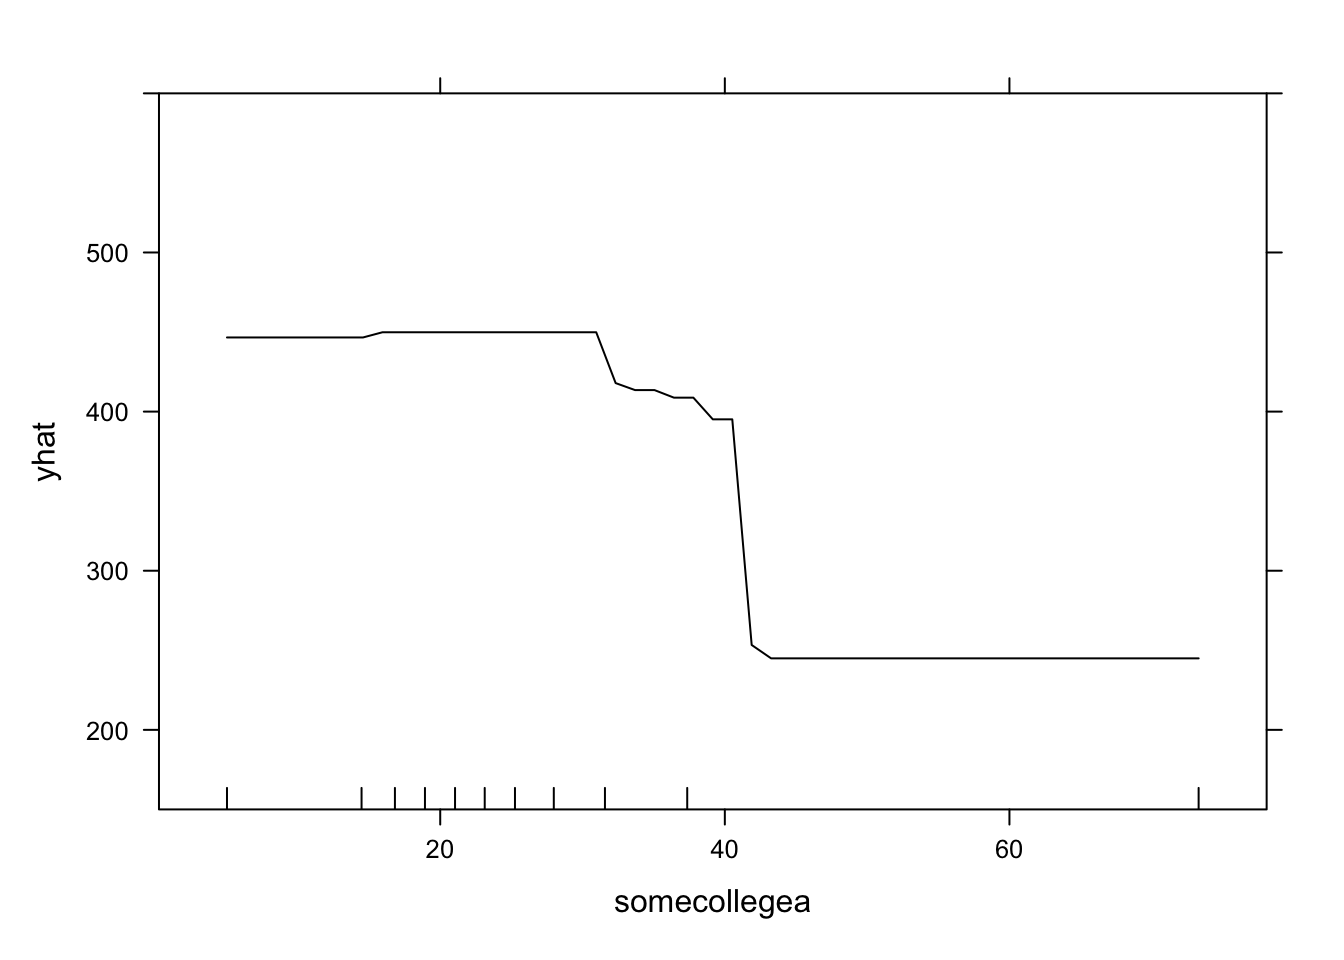
\includegraphics{3determinants_elasticity_xgbtree_newelast_files/figure-latex/unnamed-chunk-4-1.pdf}

\begin{Shaded}
\begin{Highlighting}[]
\NormalTok{xgbFitFinal}\SpecialCharTok{$}\NormalTok{bestTune}
\end{Highlighting}
\end{Shaded}

\begin{verbatim}
##    nrounds max_depth   eta gamma colsample_bytree min_child_weight subsample
## 39     576         7 0.005     0              0.5               20       0.2
\end{verbatim}

\begin{Shaded}
\begin{Highlighting}[]
\FunctionTok{stopCluster}\NormalTok{(cl)}

\FunctionTok{save}\NormalTok{(xgbFitFinal,}\AttributeTok{file=}\StringTok{"xgbFitFinal.Rdata"}\NormalTok{)}
\end{Highlighting}
\end{Shaded}

Results:

\begin{Shaded}
\begin{Highlighting}[]
\FunctionTok{load}\NormalTok{(}\AttributeTok{file=}\StringTok{"YPLLanalytic.Rdata"}\NormalTok{)}
\FunctionTok{load}\NormalTok{(}\AttributeTok{file =} \StringTok{"xgbFitFinal.Rdata"}\NormalTok{)}

\FunctionTok{plot}\NormalTok{(}\FunctionTok{varImp}\NormalTok{(xgbFitFinal))}
\end{Highlighting}
\end{Shaded}

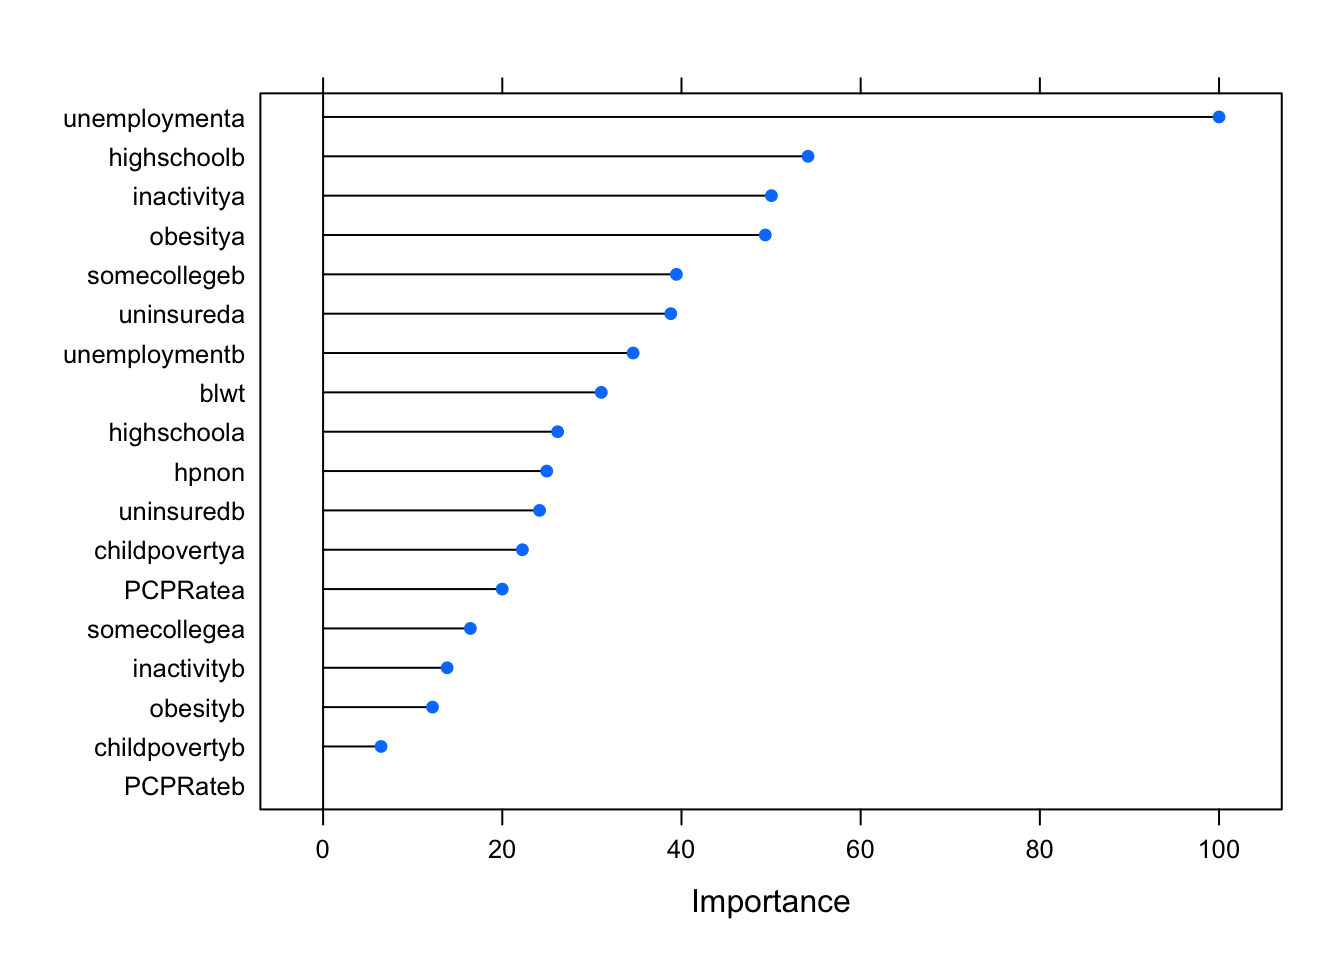
\includegraphics{3determinants_elasticity_xgbtree_newelast_files/figure-latex/unnamed-chunk-5-1.pdf}

\begin{Shaded}
\begin{Highlighting}[]
\NormalTok{vi}\OtherTok{=}\FunctionTok{varImp}\NormalTok{(xgbFitFinal)}
\NormalTok{vi}\SpecialCharTok{$}\NormalTok{importance}
\end{Highlighting}
\end{Shaded}

\begin{verbatim}
##                  Overall
## obesitya      100.000000
## inactivitya    88.772228
## somecollegea   88.168302
## PCPRateb       60.578163
## inactivityb    58.391528
## childpovertya  57.927225
## hpnon          57.030086
## highschoola    55.004340
## uninsureda     53.720164
## highschoolb    50.112562
## PCPRatea       49.386681
## unemploymenta  46.582051
## somecollegeb   43.606689
## blwt           39.858873
## obesityb       39.850189
## childpovertyb  19.422004
## uninsuredb      8.052255
## unemploymentb   0.000000
\end{verbatim}

\begin{Shaded}
\begin{Highlighting}[]
\NormalTok{xgbFitFinal}
\end{Highlighting}
\end{Shaded}

\begin{verbatim}
## eXtreme Gradient Boosting 
## 
## 2509 samples
##   18 predictor
## 
## No pre-processing
## Resampling: Cross-Validated (10 fold, repeated 10 times) 
## Summary of sample sizes: 2259, 2258, 2258, 2258, 2259, 2258, ... 
## Resampling results across tuning parameters:
## 
##   nrounds  RMSE      Rsquared    MAE     
##   500      1089.851  0.02950927  779.6507
##   502      1089.824  0.02953262  779.6333
##   504      1089.795  0.02954632  779.6084
##   506      1089.777  0.02955068  779.5970
##   508      1089.726  0.02960608  779.5757
##   510      1089.728  0.02955611  779.5796
##   512      1089.709  0.02956211  779.5730
##   514      1089.687  0.02957507  779.5708
##   516      1089.670  0.02957168  779.5568
##   518      1089.671  0.02955039  779.5548
##   520      1089.661  0.02953098  779.5451
##   522      1089.635  0.02955591  779.5312
##   524      1089.611  0.02957802  779.5247
##   526      1089.563  0.02963837  779.4881
##   528      1089.562  0.02961942  779.4907
##   530      1089.548  0.02963361  779.4794
##   532      1089.526  0.02964628  779.4655
##   534      1089.499  0.02965325  779.4498
##   536      1089.471  0.02968219  779.4234
##   538      1089.476  0.02965969  779.4225
##   540      1089.459  0.02968307  779.4011
##   542      1089.448  0.02970502  779.4051
##   544      1089.433  0.02971258  779.3936
##   546      1089.453  0.02965811  779.4043
##   548      1089.409  0.02971190  779.3666
##   550      1089.399  0.02970951  779.3552
##   552      1089.363  0.02975816  779.3274
##   554      1089.370  0.02973438  779.3402
##   556      1089.356  0.02974686  779.3198
##   558      1089.325  0.02979144  779.2891
##   560      1089.318  0.02978840  779.2858
##   562      1089.313  0.02978528  779.2697
##   564      1089.297  0.02979120  779.2574
##   566      1089.269  0.02983674  779.2354
##   568      1089.269  0.02983018  779.2329
##   570      1089.248  0.02984857  779.2270
##   572      1089.228  0.02986549  779.2204
##   574      1089.206  0.02989790  779.1958
##   576      1089.177  0.02993063  779.1761
##   578      1089.191  0.02990882  779.1823
##   580      1089.193  0.02990012  779.1823
##   582      1089.207  0.02985788  779.2069
##   584      1089.210  0.02983693  779.2141
##   586      1089.198  0.02987002  779.2167
##   588      1089.205  0.02985623  779.2309
##   590      1089.216  0.02983025  779.2398
##   592      1089.216  0.02982504  779.2428
##   594      1089.203  0.02983931  779.2392
##   596      1089.207  0.02982265  779.2540
##   598      1089.201  0.02982628  779.2407
##   600      1089.214  0.02980098  779.2501
##   602      1089.235  0.02976431  779.2631
##   604      1089.264  0.02970339  779.2806
##   606      1089.252  0.02972357  779.2840
##   608      1089.253  0.02971334  779.2787
##   610      1089.263  0.02969112  779.2887
##   612      1089.240  0.02971430  779.2803
##   614      1089.248  0.02969926  779.2713
##   616      1089.237  0.02971580  779.2594
##   618      1089.236  0.02971987  779.2547
##   620      1089.252  0.02968986  779.2692
##   622      1089.266  0.02966190  779.2846
##   624      1089.268  0.02966561  779.2881
##   626      1089.277  0.02965476  779.2996
##   628      1089.257  0.02969646  779.3043
##   630      1089.246  0.02970701  779.2985
##   632      1089.260  0.02967930  779.3208
##   634      1089.298  0.02962410  779.3465
##   636      1089.303  0.02960992  779.3552
##   638      1089.296  0.02962982  779.3417
##   640      1089.265  0.02967679  779.3261
##   642      1089.271  0.02966479  779.3428
##   644      1089.289  0.02966576  779.3714
##   646      1089.293  0.02966442  779.3724
##   648      1089.306  0.02966532  779.3708
##   650      1089.316  0.02965095  779.3774
##   652      1089.299  0.02969356  779.3580
##   654      1089.306  0.02969807  779.3554
##   656      1089.323  0.02966414  779.3681
##   658      1089.330  0.02966562  779.3846
##   660      1089.361  0.02961481  779.4151
##   662      1089.361  0.02961098  779.4247
##   664      1089.366  0.02960398  779.4407
##   666      1089.353  0.02962163  779.4277
##   668      1089.346  0.02963284  779.4290
##   670      1089.333  0.02964888  779.4244
##   672      1089.342  0.02963171  779.4353
##   674      1089.319  0.02967121  779.4352
##   676      1089.338  0.02963037  779.4488
##   678      1089.320  0.02964777  779.4368
##   680      1089.316  0.02965525  779.4337
##   682      1089.338  0.02962640  779.4484
##   684      1089.357  0.02959830  779.4575
##   686      1089.359  0.02960974  779.4652
##   688      1089.365  0.02960742  779.4639
##   690      1089.365  0.02961497  779.4588
##   692      1089.380  0.02959577  779.4729
##   694      1089.391  0.02959433  779.4730
##   696      1089.397  0.02959123  779.4883
##   698      1089.396  0.02960269  779.4876
##   700      1089.404  0.02958937  779.4925
## 
## Tuning parameter 'max_depth' was held constant at a value of 7
## Tuning parameter 'eta' was held constant at a value of 0.005
## Tuning parameter 'gamma' was held constant at a value of 0
## Tuning parameter 'colsample_bytree' was held constant at a value of 0.5
## Tuning parameter 'min_child_weight' was
##  held constant at a value of 20
## Tuning parameter 'subsample' was held constant at a value of 0.2
## RMSE was used to select the optimal model using the smallest value.
## The final values used for the model were nrounds = 576, max_depth = 7, eta = 0.005, gamma = 0, colsample_bytree = 0.5, min_child_weight = 20 and subsample = 0.2.
\end{verbatim}

\begin{Shaded}
\begin{Highlighting}[]
\NormalTok{xgb.pdp }\OtherTok{=} \FunctionTok{list}\NormalTok{()}
\NormalTok{res.partialplot }\OtherTok{=} \FunctionTok{list}\NormalTok{()}
\NormalTok{predvarls }\OtherTok{=} \FunctionTok{rownames}\NormalTok{(}\FunctionTok{varImp}\NormalTok{(xgbFitFinal)}\SpecialCharTok{$}\NormalTok{importance)}

\ControlFlowTok{for}\NormalTok{ (m }\ControlFlowTok{in} \DecValTok{1}\SpecialCharTok{:}\FunctionTok{length}\NormalTok{(predvarls))\{}
\NormalTok{  xgb.pdp[[m]] }\OtherTok{=} 
    \FunctionTok{partial}\NormalTok{(}
      \AttributeTok{object =}\NormalTok{ xgbFitFinal,}
      \AttributeTok{pred.var =}\NormalTok{ predvarls[[m]],}
      \AttributeTok{plot =} \ConstantTok{FALSE}\NormalTok{,}
      \AttributeTok{chull =} \ConstantTok{TRUE}\NormalTok{,}
      \AttributeTok{plot.engine =} \StringTok{"ggplot2"}
\NormalTok{    )}
\NormalTok{  res.partialplot[[m]] }\OtherTok{=} \FunctionTok{plotPartial}\NormalTok{(xgb.pdp[[m]], }\AttributeTok{rug =}\ConstantTok{TRUE}\NormalTok{, }\AttributeTok{train =}\NormalTok{ YPLLanalytic, }\AttributeTok{ylim=}\FunctionTok{c}\NormalTok{(}\DecValTok{99}\NormalTok{, }\DecValTok{601}\NormalTok{))}
\NormalTok{\}}

\ControlFlowTok{for}\NormalTok{(j }\ControlFlowTok{in} \DecValTok{1}\SpecialCharTok{:}\FunctionTok{length}\NormalTok{(predvarls))\{}
  \FunctionTok{print}\NormalTok{(res.partialplot[[j]])}
\NormalTok{\}}
\end{Highlighting}
\end{Shaded}

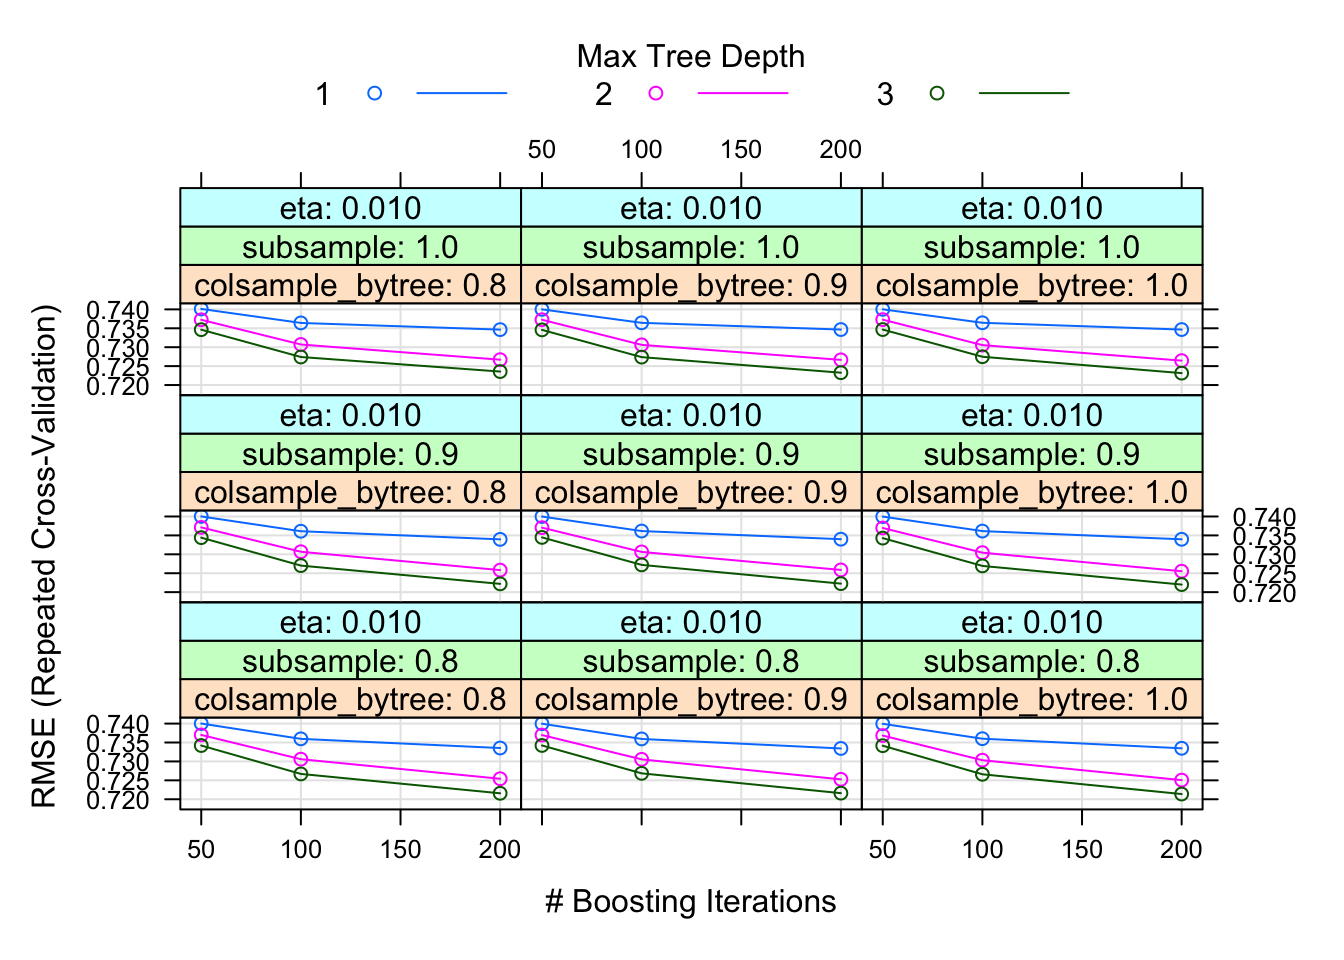
\includegraphics{3determinants_elasticity_xgbtree_newelast_files/figure-latex/unnamed-chunk-5-2.pdf}
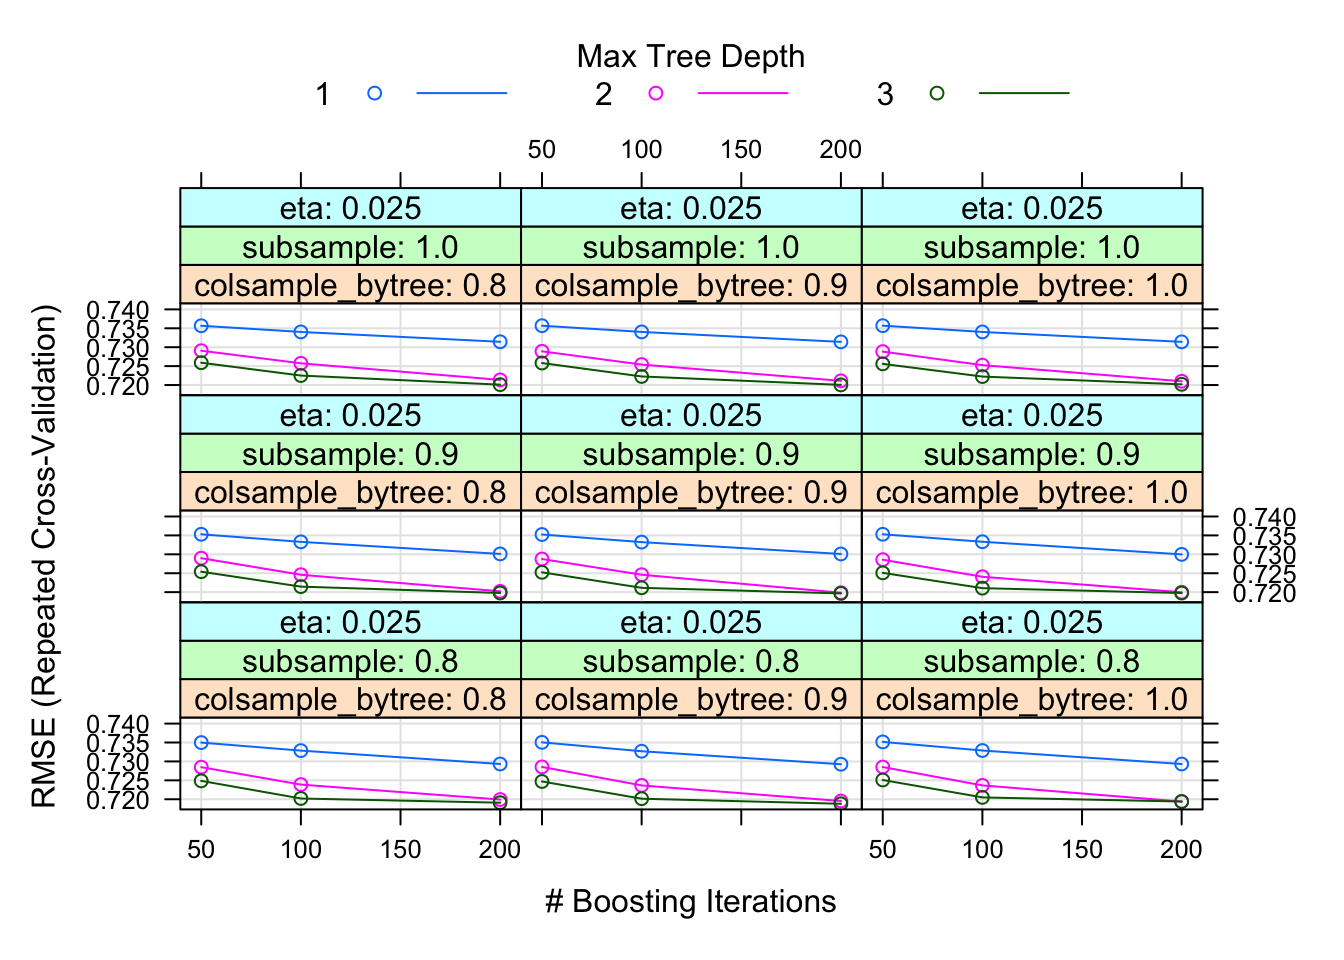
\includegraphics{3determinants_elasticity_xgbtree_newelast_files/figure-latex/unnamed-chunk-5-3.pdf}
\includegraphics{3determinants_elasticity_xgbtree_newelast_files/figure-latex/unnamed-chunk-5-4.pdf}
\includegraphics{3determinants_elasticity_xgbtree_newelast_files/figure-latex/unnamed-chunk-5-5.pdf}
\includegraphics{3determinants_elasticity_xgbtree_newelast_files/figure-latex/unnamed-chunk-5-6.pdf}
\includegraphics{3determinants_elasticity_xgbtree_newelast_files/figure-latex/unnamed-chunk-5-7.pdf}
\includegraphics{3determinants_elasticity_xgbtree_newelast_files/figure-latex/unnamed-chunk-5-8.pdf}
\includegraphics{3determinants_elasticity_xgbtree_newelast_files/figure-latex/unnamed-chunk-5-9.pdf}
\includegraphics{3determinants_elasticity_xgbtree_newelast_files/figure-latex/unnamed-chunk-5-10.pdf}
\includegraphics{3determinants_elasticity_xgbtree_newelast_files/figure-latex/unnamed-chunk-5-11.pdf}
\includegraphics{3determinants_elasticity_xgbtree_newelast_files/figure-latex/unnamed-chunk-5-12.pdf}
\includegraphics{3determinants_elasticity_xgbtree_newelast_files/figure-latex/unnamed-chunk-5-13.pdf}
\includegraphics{3determinants_elasticity_xgbtree_newelast_files/figure-latex/unnamed-chunk-5-14.pdf}
\includegraphics{3determinants_elasticity_xgbtree_newelast_files/figure-latex/unnamed-chunk-5-15.pdf}
\includegraphics{3determinants_elasticity_xgbtree_newelast_files/figure-latex/unnamed-chunk-5-16.pdf}
\includegraphics{3determinants_elasticity_xgbtree_newelast_files/figure-latex/unnamed-chunk-5-17.pdf}
\includegraphics{3determinants_elasticity_xgbtree_newelast_files/figure-latex/unnamed-chunk-5-18.pdf}
\includegraphics{3determinants_elasticity_xgbtree_newelast_files/figure-latex/unnamed-chunk-5-19.pdf}

\begin{Shaded}
\begin{Highlighting}[]
\FunctionTok{library}\NormalTok{(sfsmisc)}
\end{Highlighting}
\end{Shaded}

\begin{verbatim}
## 
## Attaching package: 'sfsmisc'
\end{verbatim}

\begin{verbatim}
## The following object is masked from 'package:Hmisc':
## 
##     errbar
\end{verbatim}

\begin{verbatim}
## The following object is masked from 'package:dplyr':
## 
##     last
\end{verbatim}

\begin{Shaded}
\begin{Highlighting}[]
\FunctionTok{library}\NormalTok{(usmap)}

\NormalTok{res\_e }\OtherTok{=} \FunctionTok{numeric}\NormalTok{(}\AttributeTok{length =} \FunctionTok{length}\NormalTok{(predvarls))}
\NormalTok{res\_semi\_e }\OtherTok{=} \FunctionTok{numeric}\NormalTok{(}\AttributeTok{length =} \FunctionTok{length}\NormalTok{(predvarls))}
\NormalTok{county\_e }\OtherTok{=} \FunctionTok{matrix}\NormalTok{(}\AttributeTok{data =} \ConstantTok{NA}\NormalTok{,}\AttributeTok{nrow =} \FunctionTok{dim}\NormalTok{(YPLLanalytic)[}\DecValTok{1}\NormalTok{],}\AttributeTok{ncol =} \FunctionTok{length}\NormalTok{(predvarls))}
\NormalTok{res.elastplot }\OtherTok{=} \FunctionTok{list}\NormalTok{()}
\NormalTok{res.semi\_elastplot }\OtherTok{=} \FunctionTok{list}\NormalTok{()}
\NormalTok{goodlist }\OtherTok{=} \FunctionTok{c}\NormalTok{(}\StringTok{"somecollegea"}\NormalTok{,}\StringTok{"somecollegeb"}\NormalTok{,}\StringTok{"PCPratea"}\NormalTok{,}\StringTok{"PCPrateb"}\NormalTok{,}\StringTok{"highschoola"}\NormalTok{,}\StringTok{"highschoolb"}\NormalTok{) }\CommentTok{\#Variables where increase is hypothesized to reduce YPLLdif}

\ControlFlowTok{for}\NormalTok{ (j }\ControlFlowTok{in} \DecValTok{1}\SpecialCharTok{:}\FunctionTok{length}\NormalTok{(predvarls)) \{}
\NormalTok{  sm\_pdp\_j }\OtherTok{=} \FunctionTok{smooth.spline}\NormalTok{(}\AttributeTok{x =}\NormalTok{ xgb.pdp[[j]][, }\DecValTok{1}\NormalTok{], }\AttributeTok{y =}\NormalTok{ xgb.pdp[[j]][, }\DecValTok{2}\NormalTok{], }\AttributeTok{df =} \DecValTok{5}\NormalTok{) }\CommentTok{\#Smooth partial dependency of YPLL on predictor j}
\NormalTok{  d\_pdp\_d\_j }\OtherTok{=} \FunctionTok{D1tr}\NormalTok{(}\AttributeTok{y =}\NormalTok{ sm\_pdp\_j}\SpecialCharTok{$}\NormalTok{y, }\AttributeTok{x =}\NormalTok{ sm\_pdp\_j}\SpecialCharTok{$}\NormalTok{x) }\CommentTok{\#Derivative of smoothed partial dependency of YPLL on predictor j}
\NormalTok{  e\_pdp\_j }\OtherTok{=}\NormalTok{ (sm\_pdp\_j}\SpecialCharTok{$}\NormalTok{x }\SpecialCharTok{/}\NormalTok{ sm\_pdp\_j}\SpecialCharTok{$}\NormalTok{y) }\SpecialCharTok{*}\NormalTok{ d\_pdp\_d\_j }\CommentTok{\#Elasticity of YPLL with respect to predictor j}
  \FunctionTok{plot}\NormalTok{(}
\NormalTok{    sm\_pdp\_j}\SpecialCharTok{$}\NormalTok{x,}
\NormalTok{    e\_pdp\_j,}
    \AttributeTok{xlab =}\NormalTok{ predvarls[j],}
    \AttributeTok{ylab =} \StringTok{"Elasticity of YPLLdif"}\NormalTok{,}
    \AttributeTok{ylim =} \FunctionTok{c}\NormalTok{(}\SpecialCharTok{{-}}\DecValTok{1}\NormalTok{, }\DecValTok{1}\NormalTok{)}
\NormalTok{  )}
\NormalTok{  interp.elast }\OtherTok{=} \FunctionTok{approxfun}\NormalTok{(}\AttributeTok{x =}\NormalTok{ sm\_pdp\_j}\SpecialCharTok{$}\NormalTok{x, }\AttributeTok{y =}\NormalTok{ e\_pdp\_j)}
\NormalTok{  res\_e[j] }\OtherTok{=} \FunctionTok{weighted.mean}\NormalTok{(}\AttributeTok{x =} \FunctionTok{interp.elast}\NormalTok{(YPLLanalytic[, predvarls[j]]), }\AttributeTok{w =}
\NormalTok{                             analyticwrace}\SpecialCharTok{$}\NormalTok{averweight)}
\NormalTok{  county\_e[, j] }\OtherTok{=} \FunctionTok{interp.elast}\NormalTok{(YPLLanalytic[, predvarls[j]])}
\NormalTok{  etest }\OtherTok{=} \FunctionTok{data.frame}\NormalTok{(}\AttributeTok{fips =}\NormalTok{ analyticwrace}\SpecialCharTok{$}\NormalTok{FIPS, }\AttributeTok{elast =}\NormalTok{ county\_e[, j])}
  \CommentTok{\# if (predvarls[j] \%in\% goodlist) \{}
  \CommentTok{\#   semi\_e\_j = {-}county\_e[, j] * abs(YPLLanalytic$YPLLdif)}
  \CommentTok{\# \} else semi\_e\_j = county\_e[, j] * abs(YPLLanalytic$YPLLdif)}
  
\NormalTok{  semi\_e\_j }\OtherTok{=}\NormalTok{ county\_e[, j] }\SpecialCharTok{*} \FunctionTok{abs}\NormalTok{(YPLLanalytic}\SpecialCharTok{$}\NormalTok{YPLLdif)}
\NormalTok{  res\_semi\_e[j]}\OtherTok{=}\FunctionTok{weighted.mean}\NormalTok{(}\AttributeTok{x =}\NormalTok{ county\_e[, j] }\SpecialCharTok{*} \FunctionTok{abs}\NormalTok{(YPLLanalytic}\SpecialCharTok{$}\NormalTok{YPLLdif), }\AttributeTok{w =}
\NormalTok{                             analyticwrace}\SpecialCharTok{$}\NormalTok{averweight)}
  
\NormalTok{  semi\_etest }\OtherTok{=} \FunctionTok{data.frame}\NormalTok{(}\AttributeTok{fips =}\NormalTok{ analyticwrace}\SpecialCharTok{$}\NormalTok{FIPS, }\AttributeTok{semi\_elast =}\NormalTok{ semi\_e\_j)}
\NormalTok{  res.elastplot[[j]] }\OtherTok{=} \FunctionTok{plot\_usmap}\NormalTok{(}\AttributeTok{regions =} \StringTok{"counties"}\NormalTok{,}
                                  \AttributeTok{data =}\NormalTok{ etest,}
                                  \AttributeTok{values =} \StringTok{"elast"}\NormalTok{) }\SpecialCharTok{+} \FunctionTok{scale\_fill\_gradientn}\NormalTok{(}
                                    \AttributeTok{colours =} \FunctionTok{c}\NormalTok{(}\StringTok{"darkgreen"}\NormalTok{, }\StringTok{"green"}\NormalTok{, }\StringTok{"white"}\NormalTok{, }\StringTok{"red"}\NormalTok{, }\StringTok{"darkred"}\NormalTok{),}
                                    \AttributeTok{na.value =} \StringTok{"gray"}\NormalTok{,}
                                    \AttributeTok{breaks =} \FunctionTok{c}\NormalTok{(}\SpecialCharTok{{-}}\DecValTok{1}\NormalTok{,}\SpecialCharTok{{-}}\NormalTok{.}\DecValTok{5}\NormalTok{, }\DecValTok{0}\NormalTok{, .}\DecValTok{5}\NormalTok{, }\DecValTok{1}\NormalTok{),}
                                    \AttributeTok{labels =} \FunctionTok{c}\NormalTok{(}\SpecialCharTok{{-}}\DecValTok{1}\NormalTok{,}\SpecialCharTok{{-}}\NormalTok{.}\DecValTok{5}\NormalTok{, }\DecValTok{0}\NormalTok{, .}\DecValTok{5}\NormalTok{, }\DecValTok{1}\NormalTok{),}
                                    \AttributeTok{limits =} \FunctionTok{c}\NormalTok{(}\SpecialCharTok{{-}}\FloatTok{1.2}\NormalTok{, }\FloatTok{1.2}\NormalTok{)}
\NormalTok{                                  ) }\SpecialCharTok{+} \FunctionTok{ggtitle}\NormalTok{(predvarls[j])}
  \FunctionTok{print}\NormalTok{(res.elastplot[[j]])}
\NormalTok{  res.semi\_elastplot[[j]] }\OtherTok{=} \FunctionTok{plot\_usmap}\NormalTok{(}\AttributeTok{regions =} \StringTok{"counties"}\NormalTok{,}
                                       \AttributeTok{data =}\NormalTok{ semi\_etest,}
                                       \AttributeTok{values =} \StringTok{"semi\_elast"}\NormalTok{) }\SpecialCharTok{+} \FunctionTok{scale\_fill\_gradientn}\NormalTok{(}
                                         \AttributeTok{colours =} \FunctionTok{c}\NormalTok{(}\StringTok{"darkgreen"}\NormalTok{, }\StringTok{"green"}\NormalTok{, }\StringTok{"white"}\NormalTok{, }\StringTok{"red"}\NormalTok{, }\StringTok{"darkred"}\NormalTok{),}
                                         \AttributeTok{na.value =} \StringTok{"gray"}\NormalTok{,}
                                         \AttributeTok{breaks =} \FunctionTok{c}\NormalTok{(}\SpecialCharTok{{-}}\DecValTok{1500}\NormalTok{,}\SpecialCharTok{{-}}\DecValTok{750}\NormalTok{,}\SpecialCharTok{{-}}\DecValTok{375}\NormalTok{, }\DecValTok{0}\NormalTok{, }\DecValTok{375}\NormalTok{, }\DecValTok{750}\NormalTok{, }\DecValTok{1500}\NormalTok{),}
                                         \AttributeTok{labels =} \FunctionTok{c}\NormalTok{(}\SpecialCharTok{{-}}\DecValTok{1500}\NormalTok{,}\SpecialCharTok{{-}}\DecValTok{750}\NormalTok{,}\SpecialCharTok{{-}}\DecValTok{375}\NormalTok{, }\DecValTok{0}\NormalTok{, }\DecValTok{375}\NormalTok{, }\DecValTok{750}\NormalTok{, }\DecValTok{1500}\NormalTok{),}
                                         \AttributeTok{limits =} \FunctionTok{c}\NormalTok{(}\SpecialCharTok{{-}}\DecValTok{3000}\NormalTok{, }\DecValTok{3000}\NormalTok{)}
\NormalTok{                                       )}\SpecialCharTok{+} \FunctionTok{ggtitle}\NormalTok{(predvarls[j])}
  \FunctionTok{print}\NormalTok{(res.semi\_elastplot[[j]])}
\NormalTok{\}}
\end{Highlighting}
\end{Shaded}

\begin{verbatim}
## Warning: Ignoring unknown parameters: linewidth
\end{verbatim}

\includegraphics{3determinants_elasticity_xgbtree_newelast_files/figure-latex/unnamed-chunk-5-20.pdf}

\begin{verbatim}
## Warning: Ignoring unknown parameters: linewidth
\end{verbatim}

\includegraphics{3determinants_elasticity_xgbtree_newelast_files/figure-latex/unnamed-chunk-5-21.pdf}
\includegraphics{3determinants_elasticity_xgbtree_newelast_files/figure-latex/unnamed-chunk-5-22.pdf}

\begin{verbatim}
## Warning: Ignoring unknown parameters: linewidth
\end{verbatim}

\includegraphics{3determinants_elasticity_xgbtree_newelast_files/figure-latex/unnamed-chunk-5-23.pdf}

\begin{verbatim}
## Warning: Ignoring unknown parameters: linewidth
\end{verbatim}

\includegraphics{3determinants_elasticity_xgbtree_newelast_files/figure-latex/unnamed-chunk-5-24.pdf}
\includegraphics{3determinants_elasticity_xgbtree_newelast_files/figure-latex/unnamed-chunk-5-25.pdf}

\begin{verbatim}
## Warning: Ignoring unknown parameters: linewidth
\end{verbatim}

\includegraphics{3determinants_elasticity_xgbtree_newelast_files/figure-latex/unnamed-chunk-5-26.pdf}

\begin{verbatim}
## Warning: Ignoring unknown parameters: linewidth
\end{verbatim}

\includegraphics{3determinants_elasticity_xgbtree_newelast_files/figure-latex/unnamed-chunk-5-27.pdf}
\includegraphics{3determinants_elasticity_xgbtree_newelast_files/figure-latex/unnamed-chunk-5-28.pdf}

\begin{verbatim}
## Warning: Ignoring unknown parameters: linewidth
\end{verbatim}

\includegraphics{3determinants_elasticity_xgbtree_newelast_files/figure-latex/unnamed-chunk-5-29.pdf}

\begin{verbatim}
## Warning: Ignoring unknown parameters: linewidth
\end{verbatim}

\includegraphics{3determinants_elasticity_xgbtree_newelast_files/figure-latex/unnamed-chunk-5-30.pdf}
\includegraphics{3determinants_elasticity_xgbtree_newelast_files/figure-latex/unnamed-chunk-5-31.pdf}

\begin{verbatim}
## Warning: Ignoring unknown parameters: linewidth
\end{verbatim}

\includegraphics{3determinants_elasticity_xgbtree_newelast_files/figure-latex/unnamed-chunk-5-32.pdf}

\begin{verbatim}
## Warning: Ignoring unknown parameters: linewidth
\end{verbatim}

\includegraphics{3determinants_elasticity_xgbtree_newelast_files/figure-latex/unnamed-chunk-5-33.pdf}
\includegraphics{3determinants_elasticity_xgbtree_newelast_files/figure-latex/unnamed-chunk-5-34.pdf}

\begin{verbatim}
## Warning: Ignoring unknown parameters: linewidth
\end{verbatim}

\includegraphics{3determinants_elasticity_xgbtree_newelast_files/figure-latex/unnamed-chunk-5-35.pdf}

\begin{verbatim}
## Warning: Ignoring unknown parameters: linewidth
\end{verbatim}

\includegraphics{3determinants_elasticity_xgbtree_newelast_files/figure-latex/unnamed-chunk-5-36.pdf}
\includegraphics{3determinants_elasticity_xgbtree_newelast_files/figure-latex/unnamed-chunk-5-37.pdf}

\begin{verbatim}
## Warning: Ignoring unknown parameters: linewidth
\end{verbatim}

\includegraphics{3determinants_elasticity_xgbtree_newelast_files/figure-latex/unnamed-chunk-5-38.pdf}

\begin{verbatim}
## Warning: Ignoring unknown parameters: linewidth
\end{verbatim}

\includegraphics{3determinants_elasticity_xgbtree_newelast_files/figure-latex/unnamed-chunk-5-39.pdf}
\includegraphics{3determinants_elasticity_xgbtree_newelast_files/figure-latex/unnamed-chunk-5-40.pdf}

\begin{verbatim}
## Warning: Ignoring unknown parameters: linewidth
\end{verbatim}

\includegraphics{3determinants_elasticity_xgbtree_newelast_files/figure-latex/unnamed-chunk-5-41.pdf}

\begin{verbatim}
## Warning: Ignoring unknown parameters: linewidth
\end{verbatim}

\includegraphics{3determinants_elasticity_xgbtree_newelast_files/figure-latex/unnamed-chunk-5-42.pdf}
\includegraphics{3determinants_elasticity_xgbtree_newelast_files/figure-latex/unnamed-chunk-5-43.pdf}

\begin{verbatim}
## Warning: Ignoring unknown parameters: linewidth
\end{verbatim}

\includegraphics{3determinants_elasticity_xgbtree_newelast_files/figure-latex/unnamed-chunk-5-44.pdf}

\begin{verbatim}
## Warning: Ignoring unknown parameters: linewidth
\end{verbatim}

\includegraphics{3determinants_elasticity_xgbtree_newelast_files/figure-latex/unnamed-chunk-5-45.pdf}
\includegraphics{3determinants_elasticity_xgbtree_newelast_files/figure-latex/unnamed-chunk-5-46.pdf}

\begin{verbatim}
## Warning: Ignoring unknown parameters: linewidth
\end{verbatim}

\includegraphics{3determinants_elasticity_xgbtree_newelast_files/figure-latex/unnamed-chunk-5-47.pdf}

\begin{verbatim}
## Warning: Ignoring unknown parameters: linewidth
\end{verbatim}

\includegraphics{3determinants_elasticity_xgbtree_newelast_files/figure-latex/unnamed-chunk-5-48.pdf}
\includegraphics{3determinants_elasticity_xgbtree_newelast_files/figure-latex/unnamed-chunk-5-49.pdf}

\begin{verbatim}
## Warning: Ignoring unknown parameters: linewidth
\end{verbatim}

\includegraphics{3determinants_elasticity_xgbtree_newelast_files/figure-latex/unnamed-chunk-5-50.pdf}

\begin{verbatim}
## Warning: Ignoring unknown parameters: linewidth
\end{verbatim}

\includegraphics{3determinants_elasticity_xgbtree_newelast_files/figure-latex/unnamed-chunk-5-51.pdf}
\includegraphics{3determinants_elasticity_xgbtree_newelast_files/figure-latex/unnamed-chunk-5-52.pdf}

\begin{verbatim}
## Warning: Ignoring unknown parameters: linewidth
\end{verbatim}

\includegraphics{3determinants_elasticity_xgbtree_newelast_files/figure-latex/unnamed-chunk-5-53.pdf}

\begin{verbatim}
## Warning: Ignoring unknown parameters: linewidth
\end{verbatim}

\includegraphics{3determinants_elasticity_xgbtree_newelast_files/figure-latex/unnamed-chunk-5-54.pdf}
\includegraphics{3determinants_elasticity_xgbtree_newelast_files/figure-latex/unnamed-chunk-5-55.pdf}

\begin{verbatim}
## Warning: Ignoring unknown parameters: linewidth
\end{verbatim}

\includegraphics{3determinants_elasticity_xgbtree_newelast_files/figure-latex/unnamed-chunk-5-56.pdf}

\begin{verbatim}
## Warning: Ignoring unknown parameters: linewidth
\end{verbatim}

\includegraphics{3determinants_elasticity_xgbtree_newelast_files/figure-latex/unnamed-chunk-5-57.pdf}
\includegraphics{3determinants_elasticity_xgbtree_newelast_files/figure-latex/unnamed-chunk-5-58.pdf}

\begin{verbatim}
## Warning: Ignoring unknown parameters: linewidth
\end{verbatim}

\includegraphics{3determinants_elasticity_xgbtree_newelast_files/figure-latex/unnamed-chunk-5-59.pdf}

\begin{verbatim}
## Warning: Ignoring unknown parameters: linewidth
\end{verbatim}

\includegraphics{3determinants_elasticity_xgbtree_newelast_files/figure-latex/unnamed-chunk-5-60.pdf}
\includegraphics{3determinants_elasticity_xgbtree_newelast_files/figure-latex/unnamed-chunk-5-61.pdf}

\begin{verbatim}
## Warning: Ignoring unknown parameters: linewidth
\end{verbatim}

\includegraphics{3determinants_elasticity_xgbtree_newelast_files/figure-latex/unnamed-chunk-5-62.pdf}

\begin{verbatim}
## Warning: Ignoring unknown parameters: linewidth
\end{verbatim}

\includegraphics{3determinants_elasticity_xgbtree_newelast_files/figure-latex/unnamed-chunk-5-63.pdf}
\includegraphics{3determinants_elasticity_xgbtree_newelast_files/figure-latex/unnamed-chunk-5-64.pdf}

\begin{verbatim}
## Warning: Ignoring unknown parameters: linewidth
\end{verbatim}

\includegraphics{3determinants_elasticity_xgbtree_newelast_files/figure-latex/unnamed-chunk-5-65.pdf}

\begin{verbatim}
## Warning: Ignoring unknown parameters: linewidth
\end{verbatim}

\includegraphics{3determinants_elasticity_xgbtree_newelast_files/figure-latex/unnamed-chunk-5-66.pdf}
\includegraphics{3determinants_elasticity_xgbtree_newelast_files/figure-latex/unnamed-chunk-5-67.pdf}

\begin{verbatim}
## Warning: Ignoring unknown parameters: linewidth
\end{verbatim}

\includegraphics{3determinants_elasticity_xgbtree_newelast_files/figure-latex/unnamed-chunk-5-68.pdf}

\begin{verbatim}
## Warning: Ignoring unknown parameters: linewidth
\end{verbatim}

\includegraphics{3determinants_elasticity_xgbtree_newelast_files/figure-latex/unnamed-chunk-5-69.pdf}
\includegraphics{3determinants_elasticity_xgbtree_newelast_files/figure-latex/unnamed-chunk-5-70.pdf}

\begin{verbatim}
## Warning: Ignoring unknown parameters: linewidth
\end{verbatim}

\includegraphics{3determinants_elasticity_xgbtree_newelast_files/figure-latex/unnamed-chunk-5-71.pdf}

\begin{verbatim}
## Warning: Ignoring unknown parameters: linewidth
\end{verbatim}

\includegraphics{3determinants_elasticity_xgbtree_newelast_files/figure-latex/unnamed-chunk-5-72.pdf}
\includegraphics{3determinants_elasticity_xgbtree_newelast_files/figure-latex/unnamed-chunk-5-73.pdf}

\begin{Shaded}
\begin{Highlighting}[]
\FunctionTok{print}\NormalTok{(}\FunctionTok{cbind}\NormalTok{(predvarls,res\_e)) }\CommentTok{\#Overall elasticity results}
\end{Highlighting}
\end{Shaded}

\begin{verbatim}
##       predvarls       res_e                 
##  [1,] "obesitya"      "0.722628703573935"   
##  [2,] "inactivitya"   "0.370187562607025"   
##  [3,] "somecollegea"  "-0.259859798699842"  
##  [4,] "PCPRateb"      "-0.00423301209769754"
##  [5,] "inactivityb"   "-0.00427052706075375"
##  [6,] "childpovertya" "0.187478719322619"   
##  [7,] "hpnon"         "0.0201177261337519"  
##  [8,] "highschoola"   "-0.0400321326226932" 
##  [9,] "uninsureda"    "-0.239355491732303"  
## [10,] "highschoolb"   "-0.0112087380758103" 
## [11,] "PCPRatea"      "0.0399755131094835"  
## [12,] "unemploymenta" "0.277642883561138"   
## [13,] "somecollegeb"  "-0.0526149802345273" 
## [14,] "blwt"          "-0.00704662253025246"
## [15,] "obesityb"      "0.037059867239215"   
## [16,] "childpovertyb" "-0.0104389801824501" 
## [17,] "uninsuredb"    "0.00380738793305452" 
## [18,] "unemploymentb" "0.0150438495678506"
\end{verbatim}

\begin{Shaded}
\begin{Highlighting}[]
\FunctionTok{print}\NormalTok{(}\FunctionTok{cbind}\NormalTok{(predvarls,res\_semi\_e)) }\CommentTok{\#semi elasticity results}
\end{Highlighting}
\end{Shaded}

\begin{verbatim}
##       predvarls       res_semi_e         
##  [1,] "obesitya"      "522.65128400551"  
##  [2,] "inactivitya"   "241.663163605211" 
##  [3,] "somecollegea"  "-138.658803621263"
##  [4,] "PCPRateb"      "-2.43694527315993"
##  [5,] "inactivityb"   "-2.06347207566088"
##  [6,] "childpovertya" "132.046718025043" 
##  [7,] "hpnon"         "15.6972640274671" 
##  [8,] "highschoola"   "-27.1175971504716"
##  [9,] "uninsureda"    "-166.978743556677"
## [10,] "highschoolb"   "-7.51616137709872"
## [11,] "PCPRatea"      "24.2266195080033" 
## [12,] "unemploymenta" "183.322017382117" 
## [13,] "somecollegeb"  "-42.7653873332059"
## [14,] "blwt"          "-7.71637768114674"
## [15,] "obesityb"      "28.4553443468538" 
## [16,] "childpovertyb" "-7.34847169099488"
## [17,] "uninsuredb"    "2.25357146884707" 
## [18,] "unemploymentb" "9.94443943601385"
\end{verbatim}

\end{document}
